\documentclass{article}[14pts]
\usepackage[utf8]{inputenc}
%% Incluir gráficos
\usepackage{graphicx}
%% Incluir links entre páginas y contenidos %%
\usepackage{lastpage}
%% Nombres de figures, contents, referencias, etc. en español %%
\usepackage[spanish,es-tabla]{babel}
\usepackage{subcaption}
%% Para agregar lista de figuras y tablas de contenidos en el índice.
\usepackage{tocbibind}
%% Paquetes matemáticos
\usepackage{amsmath,amssymb,amsthm,textcomp}
\usepackage{glossaries} %% Glosarios
%% Figuras
\usepackage{float}
\usepackage{pythonhighlight}
\usepackage[margin=1in]{geometry}
\usepackage{color}
\usepackage{fancyvrb}
\usepackage{listings}
\usepackage{xcolor}

% useful packages
\usepackage[colorlinks=true, allcolors=blue]{hyperref}
\providecommand{\abs}[1]{\lvert#1\rvert}
\providecommand{\norm}[1]{\lVert#1\rVert}

%Nuevos comandos para definiciones, teoremas y cosas
\newtheorem{definicion}{Definición}
\newtheorem{teo}{Teorema}

%Códigos
\lstset{
  language=Python,
  frame=none,
  frameround=fttt,
  framesep=5pt,
  basicstyle=\small\ttfamily,
  keywordstyle=\color{blue},
  commentstyle=\color{gray},
  backgroundcolor=\color{gray!10},
  rulecolor=\color{black}
}


% Para referencias 
\usepackage[backend=biber, style=numeric, citestyle=numeric, sorting=nyt, maxcitenames=1, maxbibnames=99]{biblatex}
\defbibheading{bibliography}[\refname]{}
\addbibresource{bibliografia.bib}

\title{Informe de Práctica I, II y III}
\author{Lourdes Mella Miranda}
\date{Marzo 2024}

% Encabezados y pies de página personalizados %%------------------%
\usepackage{fancyhdr}
\pagestyle{fancy}
\lhead{}
\chead{}
\rhead{} %% \vspace*{-1cm}
\lfoot{}
\cfoot{}
\rfoot{Página \thepage\,de \pageref*{LastPage}}
\renewcommand{\headrulewidth}{0pt}
\renewcommand{\footrulewidth}{0pt}
\setlength{\parskip}{0.35em}


%-------------------------------------------------------------------------------------------------------------------------------------------------------------
\begin{document}
\begin{titlepage}
\begin{center}


\includegraphics[width=0.3\textwidth]{images/logo_usach.png}\\[1cm]


{\large Universidad de Santiago de Chile.}\\[0.5cm]
{\large Facultad de Ciencia.}\\[0.5cm]
{\large Departamento de Matemáticas y Ciencia de la Computación.}\\[0.5cm]

{\large Ingeniería Matemática.}\\[0.5cm]

% Title
\rule{\linewidth}{0.5mm} \\[0.4cm]
{ \huge \bfseries Informe de Práctica Profesional. \\[0.4cm] }
\rule{\linewidth}{0.5mm} \\[1.5cm]

% Author and supervisor
\noindent
\begin{minipage}{0.4\textwidth}
  \begin{flushleft} \large
  \end{flushleft}
\end{minipage}%
\begin{minipage}{0.4\textwidth}
  \begin{flushright} \large
    \emph{Estudiante:} \\
   Lourdes Mella Miranda
  \end{flushright}
\end{minipage}
\\

\vspace{1cm}

\noindent
\begin{minipage}{0.4\textwidth}
  \begin{flushleft} \large
  \end{flushleft}
\end{minipage}%
\begin{minipage}{0.4\textwidth}
  \begin{flushright} \large
    \emph{Profesor:} \\
   Rafael Labarca Briones
  \end{flushright}
\end{minipage}

\vfill

% Bottom of the page
{\large \today}
\end{center}
\end{titlepage}

%% Capítulos

\tableofcontents
%% \listoftables
%% \listoffigures
\newpage

\section{Información del practicante y la empresa}

  \subsection{Datos de la empresa}

    \begin{tabular}{r l}
        Razón social & EY SERVICIOS PROFESIONALES DE AUDITORIA Y ASESORIAS LIMITADA.\\
        Rut & 77.802.430-6.\\
      Tipo de Sociedad & Sociedad de responsabilidad limitada.\\
      Ubicación & Presidente Riesco 5435 piso 4, Las Condes, Santiago de Chile.\\

    \end{tabular}

  \subsection{Datos del practicante}

    \begin{tabular}{r l}
      Nombre & Lourdes Raquel del Pilar Mella Miranda.\\ 
      Rut & 20.055.740-9.\\
      Mail & lourdes.mella@usach.cl\\
      Institución & Universidad de Santiago de Chile.\\
      Facultad & Facultad de Ciencia.\\
      Departamento & Departamento de Matemática y Ciencia de la Computación.\\
      Carrera & Ingeniería Matemática.\\
      Tipo de práctica & Profesional.\\
      Cargo & Data Scientist practicante.\\
      Área & Consultoría\\
      Equipo & Digital Data \& Analytics.\\
      Supervisor & Loreto Sánchez\\
      Título supervisor & Ing. Civil Acústica, UACh.\\
      Postgrado supervisor & Candidata a Doctora en Ingeniería Eléctrica.

    \end{tabular}

\section{Acerca de la empresa.}

  \subsection{EY Chile}

  Fundada en 2007, EY Chile es la filial chilena de Ernst \& Young (EY), una de las principales firmas de servicios 
  profesionales a nivel mundial. Con una destacada presencia en el ámbito de la consultoría, auditoría, impuestos 
  y asesoramiento financiero, se ha consolidado como una entidad líder en el mercado. 

  Recientemente, EY fue reconocida como la décima mejor empresa para trabajar en América Latina en 2023, según la 
  lista de Great Place to Work. Este logro destaca el compromiso continuo de la firma con la calidad laboral y el 
  bienestar de sus colaboradores. Esta firma cuenta con una red global que abarca más de 700 ubicaciones en más de 150 países; asimismo, su filial chilena tiene presencia con oficinas estratégicas en Santiago, Viña del Mar, Concepción y Puerto Montt.

  Para garantizar una atención especializada, EY Chile organiza sus servicios a través de diversas divisiones, 
  brindando soluciones a una amplia gama de clientes. Estas divisiones incluyen:

    \begin{itemize}

        \item \textbf{Estrategia y transacciones:} EY destaca en la prestación de servicios de estrategia y 
        transacciones. Su enfoque personalizado a cada cliente, respaldado por una amplia experiencia multinacional, utiliza técnicas analíticas para impulsar decisiones de alto impacto. Esta firma se especializa en estrategia corporativa, asignación de capital y ejecución de transacciones, brindando apoyo a clientes de diversos sectores en la creación y preservación de valor. 

        \item \textbf{Consultoría:} La consultoría en EY impulsa la transformación empresarial al integrar 
        estratégicamente personas, tecnología e innovación. Adaptándose a la rápida evolución del entorno laboral, la firma fomenta comportamientos innovadores y colaborativos para abordar desafíos clave en la actualidad. Al priorizar a las personas, aprovechar la tecnología de manera ágil y promover la innovación, EY genera valor a largo plazo para individuos, empresas y la sociedad en general.

        \item \textbf{Auditoría y finanzas:} Los equipos de Auditoría y Finanzas de EY en Chile desempeñan un papel 
        crucial al servir al interés público, promoviendo la confianza en empresas y mercados de capitales. A través de servicios que abarcan auditoría, asesoría en contabilidad financiera y análisis forense, EY aborda riesgos, complejidades y oportunidades, protegiendo y promoviendo un valor sostenible a largo plazo.

        \item \textbf{Impuestos:} Los profesionales de impuestos de EY en Chile ofrecen servicios completos en todas las disciplinas tributarias. Con competencias en impuestos empresariales, internacionales, sobre transacciones y legislación, EY combina conocimiento y experiencia para ayudar a las empresas a prosperar en un entorno de cambios rápidos.

        \item \textbf{EY Law - Servicios legales:} EY Law proporciona orientación detallada para abordar el complejo entorno legal global. Con un enfoque multidisciplinario, la firma ayuda a reducir la brecha entre asesores de negocios y legales, aumentando la eficiencia y velocidad de comercialización. Su enfoque centrado en el sector brinda asesoría integrada y detallada, con servicios gestionados de manera centralizada para empresas en todo el mundo.
        
        \end{itemize}

  \subsection{Visión general}  

    \begin{itemize}

      \item[\textbf{Misión:}] ``Construir un mejor mundo de negocios mediante servicios de calidad que fomentan la 
      confianza en los mercados y el desarrollo de líderes excepcionales.''

      \item[\textbf{Visión:}] ``En EY, estamos construyendo el lugar de trabajo del futuro, más inteligente, inclusivo y 
      dinámico, adaptándonos al cambio y promoviendo el crecimiento económico más inclusivo.''

      \item[\textbf{Valores:}] 

    \begin{enumerate}
        
        \item[i)] \emph{Integridad:} ``Demostramos honestidad y coherencia en todas nuestras acciones y decisiones'' 
        
        \item[ii)] \emph{Respeto:} ``Valoramos y reconocemos las diferencias individuales, fomentando un ambiente 
        inclusivo y de respeto mutuo.'' 

        \item[iii)] \emph{Trabajo en equipo:} ``Colaboramos de manera efectiva, reconociendo la importancia del trabajo conjunto para lograr el éxito.''

        \item[iv)] \emph{Inclusión:} ``Valoramos y potenciamos las diferencias individuales, reconociendo que la 
        diversidad impulsa la innovación y contribuye al éxito a largo plazo en el mercado global.''

        \item[v)] \emph{Energía:}  ``Demostramos vitalidad y pasión en nuestra labor diaria, buscando continuamente 
        formas de agregar valor.''

        \item[vi)] \emph{Entusiasmo:} ``Mostramos un entusiasmo positivo hacia nuestros colegas, clientes y desafíos profesionales.''

        \item[vii)] \emph{Coraje para liderar:}  ``Nos destacamos por asumir la responsabilidad y liderar con valentía, basándonos en principios éticos y en hacer lo correcto en nuestras relaciones.''
      
    \end{enumerate}

    \item[\textbf{Logo:}]
  \end{itemize} 

      \begin{center}
          
\includegraphics[scale=0.15]{images/EY_logo.png}
      \end{center}

\section{Aspectos generales y contextualización}

  \subsection{Marco conceptual}

    \subsubsection{Industria 4.0}
      
    La industria ha experimentado una evolución constante, desde sus primeras etapas hasta la revolución actual de la Industria 4.0. Cada fase ha marcado un hito en el desarrollo de nuevas tecnologías y enfoques de producción, 
    llevándonos a la actual convergencia de tecnologías digitales. A continuación, presentamos una ilustración que 
    representa la evolución industrial a lo largo del tiempo:

      \begin{center}
        \begin{figure}[h]
            \centering
            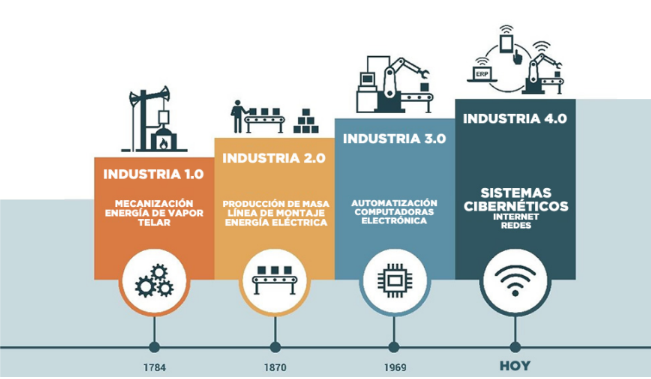
\includegraphics[width=0.8\textwidth]{images/industria.png}
            \caption{Evolución Industrial}
        \end{figure}    
      \end{center}

    Hoy en día, nos encontramos inmersos en la era de la Industria 4.0, una revolución industrial impulsada por el 
    impacto de la tecnología digital y el procesamiento avanzado de datos. Este cambio de paradigma ha dado origen a las denominadas fábricas inteligentes, redefiniendo por completo los modelos de producción y generando una creciente automatización que impulsa la productividad a niveles sin precedentes.

    En esta nueva era industrial, es crucial comprender conceptos clave que impulsan la transformación. Definamos 
    algunos de estos términos fundamentales:

    \begin{itemize}

        \item \textbf{Internet de las Cosas (IoT):} Se refiere a la interconexión de dispositivos y sistemas a través de la red, permitiendo la recopilación y el intercambio de datos en tiempo real. El IoT es un componente esencial para la operación eficiente de fábricas inteligentes.

        \item \textbf{Big Data:} Aborda la gestión y análisis de conjuntos de datos masivos. En la Industria 4.0, el Big Data juega un papel crucial al procesar la gran cantidad de información generada por sensores y dispositivos conectados, proporcionando conclusiones valiosas para la toma de decisiones. 
      
        \item \textbf{Cloud computing:} La computación en la nube ofrece almacenamiento y procesamiento de datos de 
        forma remota, permitiendo el acceso a recursos computacionales escalables. De este modo, se facilita la 
        gestión eficiente de grandes cantidades de datos y servicios.
        
    \end{itemize}

    \subsubsection{Estrategias de mantenimiento industrial}

    En el ámbito industrial, la gestión del mantenimiento se ha transformado significativamente debido al desarrollo tecnológico de los equipos de control y medida. A continuación definimos los tres principales tipos de mantenimiento:

    \begin{itemize}

        \item \textbf{Mantenimiento Correctivo:} Actúa tras la ocurrencia de una avería, minimizando tiempos de 
        detención de maquinaria. Sin embargo, puede generar tiempos muertos no planificados.

        \item \textbf{Mantenimiento Preventivo:} Realiza ajustes programados para mantener herramientas y equipos en condiciones seguras. Aunque permite una planificación anticipada, puede dar lugar a intervenciones 
        innecesarias y costos constantes.

        \item \textbf{Mantenimiento Predictivo:} Evalúa el estado de la maquinaria en tiempo real basándose en su 
        condición. Utiliza sensores para recopilar datos, luego procesa esta información para determinar la necesidad de intervención. Logra optimizar la fiabilidad y disponibilidad de la maquinaria a un costo mínimo.
        
    \end{itemize}

      \begin{center}
        \begin{figure}[h]
          \centering
          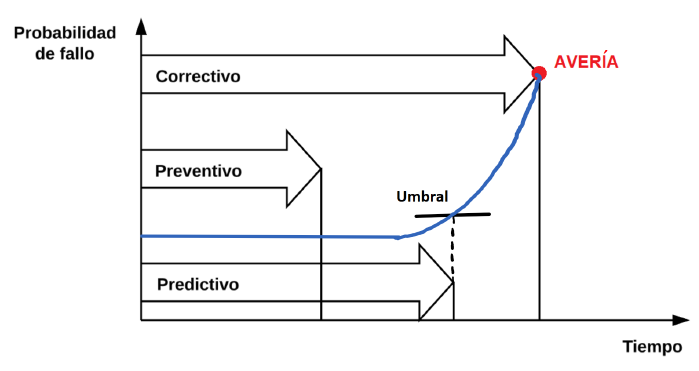
\includegraphics[width=0.7\textwidth]{images/mantenimiento.png}
          \caption{Tipos de mantenimiento}
        \end{figure}    
      \end{center}
      
    Con lo expuesto anteriormente, se evidencia la estrecha relación entre el mantenimiento predictivo y la Industria 4.0. Este enfoque de mantenimiento, al evaluar en tiempo real el estado de la maquinaria basándose en datos recopilados por sensores, se alinea perfectamente con la interconexión de dispositivos propuesta por el Internet de las Cosas (IoT). Sin duda, la capacidad de recopilar, procesar y analizar grandes conjuntos de datos, conocida como Big Data, se convierte en un pilar fundamental para el éxito del mantenimiento predictivo. Además, la adopción de tecnologías como la computación en la nube (Cloud Computing) potencia la eficiencia operativa al proporcionar un entorno escalable y accesible para el procesamiento de datos.

    \subsubsection{Machine learning}

    El machine learning es una rama de la inteligencia artificial que se centra en el desarrollo de algoritmos y 
    modelos capaces de aprender patrones y realizar tareas específicas sin una programación explícita. En lugar de 
    seguir instrucciones predefinidas, los algoritmos de machine learning utilizan datos para mejorar su rendimiento y realizar predicciones o tomar decisiones. 

    El proceso de aprendizaje de un algoritmo de machine learning se compone de varias etapas. Inicia con la 
    preparación de datos, donde se recopilan y estructuras los datos necesarios, seguido por la selección de 
    características clave. Posteriormente, se dividen los datos en conjuntos de entrenamiento y prueba. La elección 
    y entrenamiento del modelo son fases cruciales, seguidas de la validación y ajuste para optimizar su rendimiento. 

    La evaluación del modelo es fundamental antes de su implementación en el entorno de producción, donde se 
    monitorea continuamente para garantizar su eficacia y adaptibilidad a lo largo del tiempo. Este proceso iterativo permite que el modelo evolucione y mejore su capacidad predictiva.

      \begin{center}
        \begin{figure}[h]
          \centering
          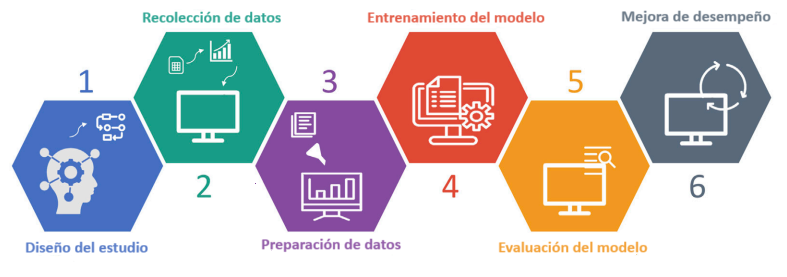
\includegraphics[width=0.7\textwidth]{images/workflowml.png}
          \caption{Flujo general del proceso de aprendizaje de un algoritmo de machine learning.}
        \end{figure}    
      \end{center}

    Las aplicaciones del machine learning son amplias y se extienden a diversas áreas, incluyendo la industria, la 
    medicina y las finanzas. En el contexto de la detección de anomalías, el aprendizaje automático juega un rol 
    crucial, ya que estos algoritmos pueden identificar patrones inusuales en conjuntos de datos, señalando 
    comportamientos atípicos.

    Así, al utilizar modelos de machine learning para la detección de anomalías, podemos anticipar posibles fallos 
    en la maquinaria industrial. Al utilizar datos provenientes de sensores y mediciones, los algoritmos pueden 
    aprender los patrones normales de operación y destacar desviaciones significativas, permitiendo prever la 
    necesidad de intervenciones de mantenimiento. 

  \subsection{Contexto}

  El equipo de Digital Data \& Analytics del área de consultoría de EY Chile está compuesto por profesionales
  especializados en ciencia e ingeniería de datos, así como desarrolladores de software, junto con otros roles clave en la gestión de proyectos. Durante mi periodo de práctica profesional, desempeñé el rol de Data Scientist en un proyecto de mantenimiento predictivo para la Corporación Nacional del Cobre de Chile (Codelco). El equipo de consultores al que me uní estaba formado por un Data Scientist, un Data Engineer y un Software Developer, quienes colaboraban estrechamente con sus contrapartes en Codelco.

  El proyecto tenía como objetivo desarrollar un sistema de alertas en el contexto del mantenimiento predictivo. Al 
  unirme al equipo, ya existía un sistema preliminar en fase de prueba y mejora antes de su implementación oficial. En este escenario, mi responsabilidad fue investigar y probar métodos alternativos al detector de anomalías asociado al sistema de alerta.

\section{Descripción general del trabajo realizado}

  \subsection{Resumen de actividades ejecutadas}

  El inicio del periodo de práctica fue destinado a estudiar conceptos y técnicas utilizadas en mantenimiento 
  predictivo. Estando ya familiarizada con el tema, se me realizó una inducción al proyecto. Este proceso consistió 
  en varias reuniones con el equipo, en donde me presentaron los aspectos generales del sistema de alertas
  desarrollado, enfatizando en el detector de anomalías utilizado para generar las alarmas. 

  Posteriormente, se me otorgaron los permisos para acceder a \textit{Databricks}, la plataforma de análisis y 
  procesamiento de datos integrada con la nube de \textit{Microsoft Azure}, utilizada como entorno principal para el desarrollo del proyecto. Inicié mi trabajo explorando el código del detector de anomalías, implementado en el 
  lenguaje de programación \textit{Python}. Simultáneamente, me integré a las actividades del equipo que operaba bajo una metodología ágil, caracterizada por reuniones diarias para informar sobre el avance del proyecto y mantener una comunicación efectiva.

  En este punto, al comprender el funcionamiento de Databricks, así como los objetivos del sistema de alertas y la dinámica del equipo, se definió que mi misión consistiría en investigar y proponer métodos alternativos al detector de anomalías. Este proceso implicó la revisión de literatura y documentación de librerías, el desarrollo de pruebas numéricas y el análisis de los resultados obtenidos. Durante todo este estudio conté con el apoyo y guía de los científicos de datos del equipo. Además, se estableció que, para concluir mi participación en el proyecto, debía presentar el trabajo realizado al equipo de Data Science del área de Analítica Avanzada de Codelco.

  \subsection{Proyecto asignado: Sistema de alertas de mantenimiento}

  La División Radomiro Tomic, ubicada en la región de Antofagasta, se especializa en la extracción y procesamiento de minerales de cobre, desempeñando un papel significativo en la producción total de Codelco. Esta división opera específicamente en una mina a tajo abierto, extrayendo minerales de cobre desde la superficie terrestre. La mina se distingue por su vasto terreno y su compromiso con la eficiencia y sostenibilidad en todas sus operaciones.

  Este proyecto surge de la necesidad de implementar una nueva estrategia de mantenimiento predictivo, que permita 
  optimizar la eficiencia y confiabilidad de las operaciones en la división. Al momento de contactar a EY, utilizaban un software de sistema de alertas de mantenimiento anticuado y costoso, por lo que el objetivo era crear un sistema propio. 

  Al incorporarme al equipo, ya se había creado un sistema de alertas que se encontraba en periodo de prueba. Las alertas generadas eran revisadas por analistas expertos en las plantas de operación, quienes las categorizaban como aceptadas o rechazadas, especificando la razón de rechazo. El sistema de alertas desarrollado, basado en la integración de sensores en componentes clave de la maquinaria 
  utilizada en las operaciones mineras como motores, reductores y poleas, tiene como elemento esencial el detector de anomalías. Este detector se define como un conjunto de reglas y métodos especializados que permiten identificar, mediante el análisis de la evolución temporal de la energía vibratoria medida en RMS (Root Mean Square amplitude) o la temperatura medida en grados Celsius, los posibles fallos en dichos componentes. La detección temprana de estas anomalías posibilita la ejecución oportuna de acciones de mantenimiento, evitando así eventuales accidentes o paros de producción no planificados.

  En el momento en que me incorporé al proyecto, el detector de anomalías utilizado estaba configurado mediante un conjunto de parámetros que determinaban la sensibilidad del algoritmo para identificar posibles fallas. Estos parámetros no se calibraban de manera automática, lo que podría resultar en una falta de adaptibilidad a cambios en las condiciones operativas y, por lo tanto, reducir la eficacia del detector. En consecuencia, se me encomendó la tarea de investigar y probar métodos alternativos al detector de anomalías existente, pensando en mejorar la capacidad del sistema para identificar potenciales averías de manera más precisa y adaptable.  

  Una vez definida mi tarea principal, colaboré con el equipo de Data Science para investigar diversas técnicas de machine learning adecuadas para la detección de anomalías en el contexto del proyecto. En este proceso, identificamos y seleccionamos dos técnicas que se centran en la identificación de puntos de cambio en la serie temporal que describe las mediciones recopiladas por los sensores instalados en la maquinaria. 

  En la próxima sección, describiré detalladamente la principal tarea que realicé durante mi práctica profesional: 
  la investigación y prueba de técnicas alternativas al detector de anomalías utilizado en el sistema de alertas del proyecto.

\section{Prueba de métodos alternativos al detector de anomalías}

  \subsection{Objetivos de la tarea}

    Con el propósito de encontrar una técnica de detección de anomalías cuyos parámetros pudieran calibrarse 
    automáticamente, se propuso llevar a cabo la evaluación de técnicas sustitutas al detector de anomalías en uso. 
    En este contexto, se fijaron los objetivos de esta labor de la siguiente manera:

      \subsubsection{Objetivo General}

        \begin{itemize}
          \item Realizar pruebas con métodos alternativos al detector de anomalías utilizado.
        \end{itemize}

      \subsubsection{Objetivos Específicos}

          \begin{itemize}
              \item Revisar la bibliografía y documentación de los métodos Offline Changepoint Detection de Ruptures y
              Trend Changepoints de Prophet.
              
              \item Diseñar y realizar pruebas numéricas con datos reales de alertas previamente generadas.
              
              \item Establecer metodologías de análisis acordes a los métodos seleccionados.
              
              \item Extraer conclusiones de los resultados obtenidos.
          \end{itemize}

  \subsection{Esquema general de las pruebas numéricas}
  
    Para llevar a cabo las pruebas, el equipo me proporcionó un notebook en Databricks, otorgándome acceso a información detallada sobre las alertas generadas por el detector de anomalías en uso. El notebook ''Prueba Nuevos Métodos DA'' ofrece acceso a datos de alertas clasificados según el tipo de componente (motor, reductor o polea) y su estado (activo o rechazado). 

    Cada alerta se identifica según el número identificador del componente en potencial falla ''i\_indicador'' y la fecha y hora en que se emitió el aviso ''id\_alert''. La lista de las alarmas emitidas e identificadas está disponible en un DataFrame llamado ``df\_info\_componente''.  Por otro lado, el registro de las mediciones de energía vibratoria en RMS junto con la hora y fecha de cada registro se almacena en el DataFrame ``df\_features\_componente''. La idea es trabajar con las series temporales de la evolución de los registros de energía vibratoria medida en RMS antes de la generación de la alerta.

    Para ilustrar,  tomemos como ejemplo la alerta con $\text{''i\_indicador''}= 25142$ y $\text{''id\_alert''} = 22-09-01\text{T}00:00:000+0000$ en los motores. Filtrando ``df\_features\_mot'' con esos valores obtenemos la serie temporal asociada y creamos su DataFrame llamado ``df\_example\_mot''.

      \begin{center}
        \begin{figure}[h]
          \centering
          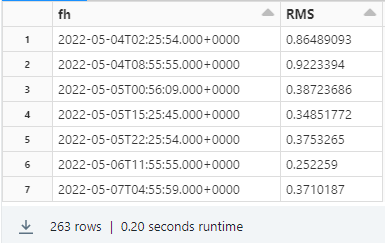
\includegraphics[width=0.4\textwidth]{images/3.png}
          \caption{Datos de la serie temporal de RMS asociada a la alerta de ejemplo. La columna ``fh'' representa la fecha y hora de medición, mientras que ``RMS'' es el valor de energía vibratoria medido.}
        \end{figure}    
      \end{center}

      \begin{center}
        \begin{figure}[h]
          \centering
          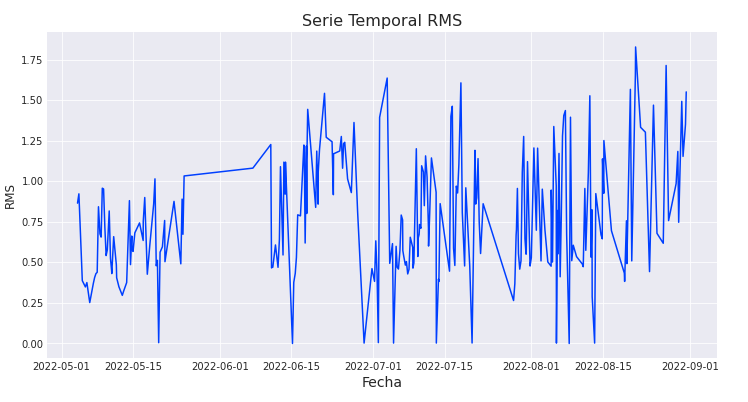
\includegraphics[width=0.6\textwidth]{images/4.png}
          \caption{Gráfico de la serie temporal de RMS asociada a la alerta de ejemplo.}
        \end{figure}    
      \end{center}
      
    Se define que el esquema general para realizar las pruebas numéricas es el siguiente:

      \begin{enumerate}

        \item Extraer la serie temporal de RMS asociada a una alerta y almacenarla en un dataframe. 
          
        \item Probar modelos de detección de puntos de cambios en estas series temporales.
          
        \item Identificar puntos de cambio y establecer el último bloque temporal. 
          
        \item Analizar el último bloque temporal para determinar si la alerta debió haber sido generada o no, según la metodología de análisis diseñada.
          
      \end{enumerate}
    
  \subsection{Offline Changepoint Detection (librería Ruptures)}

  \subsubsection{Sobre la técnica y la librería}

    La detección de puntos de cambio es una técnica utilizada en análisis de datos para identificar momentos en los cuales el comportamiento de un sistema o proceso cambia de manera significativa. Estos puntos de cambio pueden representar momentos de transición entre diferentes estados o regímenes en los datos. En este contexto, el modo offline se refiere a la capacidad de analizar un conjunto completo de datos históricos en un solo paso, en contraposición a los métodos online que procesan datos a medida que llegan, en tiempo real.

    El análisis de puntos de cambio en modo offline implica examinar un conjunto de datos que ya está completamente disponible y no cambiará en el futuro. Esto significa que se pueden aplicar algoritmos de detección de puntos de cambio que tomen en cuenta todo el historial de datos para identificar las rupturas o cambios en el comportamiento de la serie temporal.
    
    La librería Ruptures es una herramienta de Python utilizada para la detección de puntos de cambio offline en series temporales u otro tipo de datos secuenciales. Se basa en la idea de que los puntos de cambio separan los datos en diferentes segmentos que poseen distintas distribuciones estadísticas. Esta librería proporciona implementaciones eficientes de varios métodos de búsqueda de puntos de cambio. Los detalles teóricos detrás de Ruptures están disponibles en el artículo escrito por C. Truoung et. al \cite{truong2020selective}.

    Según ese estudio, para formular el problema consideramos un proceso aleatorio multivariado no estacionaria $y= \{y_{1}, \dots, y_{T}\}$ que toma valores en $\mathbb{R}^{d} \ (d \geq 1)$ y tiene $T$ muestras. Asumimos que esta señal es estacionaria por partes, es decir, algunas características del proceso cambian abruptamente en algunos instantes desconocidos $t_{1}^{*} < t_{1}^{*} < \dots < t_{k}^{*}$. La detección de puntos de cambio consiste en estimar los índices $t_{k}^{*}$. Dependiendo del contexto, el número de cambios $K^{*}$ puede ser conocido o no, en tal caso también debe ser estimado.

    Formalmente, la detección de puntos de cambio se clasifica como un problema de selección de modelos, que consiste en escoger la mejor segmentación posible $\mathcal{T}$ de acuerdo a un criterio cuantitativo $V(\mathcal{T})$ que debe ser minimizado. La eleccción de la función de criterio depende del conocimiento preliminar de la tarea. 
    
    Consideraremos que la función de criterio $V(\mathcal{T})$ para una segmentación en particular corresponde a la suma de costos de todos los segmentos que componen dicha segmentación:

      \begin{equation*}
        V(\mathcal{T}) := \sum_{k=0}^{K} c(y_{t_{k}\dots t_{k+1}})
      \end{equation*}

    donde $c(\cdot)$ es una función de costo que mide la bondad de ajuste de la subseñal $y_{t_{k}\dots t_{k+1}} = \{y_{t}\}_{t_{k}}^{t_{k+1}}$ a un modelo en específico. La mejor segmentación minimiza al criterio $V(\mathcal{T})$. Según si se conoce el número de puntos de cambio $K^{*}$, existen dos problemas a resolver:

      \begin{itemize}

        \item \textbf{Problema 1: número de cambios $K$ conocido.} Consiste en resolver el siguiente problema de optimización: 
        \begin{align*}
          \min_{\|\mathcal{T}\|= K} V(\mathcal{T}) \tag{P1} \label{eq:P1}
        \end{align*}
      
        \item \textbf{Problema 2: número de cambios $K$ desconocido.} En este caso, el problema de optimización por resolver es el siguiente:
          \begin{align*}
            \min_{\mathcal{T}} V(\mathcal{T}) \ + \text{pen}(\mathcal{T}) \text{ } \tag{P2} \label{eq:P2}
          \end{align*}
        
        donde $\text{pen}(\mathcal{T})$ es una medida apropiada de la complejidad de la segmentación $\mathcal{T}$.

      \end{itemize}
    
    Los métodos de detección de puntos de cambio encuentran una solución exacta o aproximada a \eqref{eq:P1} o a \eqref{eq:P2}. 

    Consideramos que un modelo de detección de puntos de cambio se compone de los siguientes elementos:

      \begin{enumerate}
        \item \textbf{Función de costo:} La función de costo $c(\cdot)$ mide la ``homogeneidad''. Se espera que $c(y_{a\dots b})$ sea pequeña si la sub-señal $y_{a\dots b}$ es homogénea (sin puntos de cambio) y grande si es heterogénea (con uno o varios puntos de cambio).
        
        \item \textbf{Método de búsqueda:} Corresponde al procedimiento de resolución para los problemas de optimización. Cada método busca un equilibrio entre complejidad computacional y precisión.
        
        \item \textbf{Restricción (en el número de puntos de cambio):} Cuando el número de puntos de cambio es desconocido \eqref{eq:P2}, se añade una restricción en forma de penalización por complejidad $\text{pen}(\cdot)$ para balancear la bondad de ajuste $V(\mathcal{T})$. La elección de la penalización depende de la magnitud de la cantidad de cambios a detectar: con una penalización muy baja en comparación con la bondad de ajuste resulta en la detección de muchos puntos de cambio, incluso si son producto del ruido. Por otro lado, una penalización muy alta solo detecta los puntos de cambio más significativos, o ninguno. 
      \end{enumerate}
      
    Al estudiar la tarea a realizar, se definió que se optará por utilizar métodos de regresión lineal por partes. Estos modelos son ideales para capturar cambios estructurales en el comportamiento de la serie temporal en estudio. En este contexto, existe una relación lineal entre una variable de respuesta y las covariables y cambia abruptamente en algunos instantes desconocidos. Formalmente, diremos que la señal observada $y$ sigue un modelo lineal por partes c on puntos de cambio $t_{k}^{*}$:

      \begin{equation}
        \forall t, \ t_{k}^{*} < t \leq t_{k+1}^{*}, \quad y_{t}= x_{t}^{'}u_{k} + z_{t}^{'}v + \epsilon_{t} \quad (k= 0, \dots, K^{*})
      \end{equation}
    donde $u_{k} \in \mathbb{R}^{p}$ y $v \in \mathbb{R}^{q}$ son parámetros de regresión desconocidos y $\epsilon_{t}$ es ruido. Bajo esta configuración, la señal observada se considera como una variable de respuesta unidimensional ($d=1$) y las señales $x= \{x_{t}\}_{t=1}^{T}$ y $z= \{z_{t}\}_{t=1}^{T}$ son covariables observadas, con valores en $\mathbb{R}^{p}$ y $\mathbb{R}^{q}$ respectivamente. De este modo, la detección de puntos de cambio se puede llevar a acabo ajustando un modelo de regresión lineal en cada segmento de la señal. 

    A continuación definiremos las funciones de costo asociadas a este modelo:

      \begin{itemize}

        \item \textbf{Función de costo $L1$ ($c_{L1}$):} Se basa en el criterio de mínimas desviaciones absolutas y frecuentemente se utiliza cuando los datos tienen distribuciones de ruido con colas pesadas. Para una señal $y$ y covariables $x$ y $z$ , la función de costo $c_{L1}$ se define de la siguiente forma:
          
          \begin{equation}
            c_{L1}(y_{a\dots b}) = \min_{u \in \mathbb{R}^{p}, v \in \mathbb{R}^{q}} \sum_{t= a+1}^{b} \abs{y_{t} - x_{t}^{'} - z_{t}^{'}}.
          \end{equation}
          
        \item \textbf{Función de costo lineal ($c_{lineal}$):} Esta función está formulada a partir del criterio de mínimos cuadrados y es más eficiente computacionalmente que $c_{L1}$. Está dada por:
          
          \begin{equation}
            c_{lineal}(y_{a\dots b}) = \min_{u \in \mathbb{R}^{p}, v \in \mathbb{R}^{q}} \sum_{t= a+1}^{b} (y_{t} - x_{t}^{'} - z_{t}^{'})^{2}.
          \end{equation}
          
        \item \textbf{Función de costo lineal continua ($c_{clineal}$):}  Dado un conjunto de índices $t_{k} (k =1, \dots, K)$, una función spline lineal $f$ es tal que:
        
          \begin{enumerate}
            \item $f$ es afín en cada intervalo $t_{k} \dots t_{k+1}$, es decir, $f(t)= \alpha_{k}(t-t_{k})+ \beta_{k} (\alpha_{k}, \beta_{k} \in \mathbb{R}^{d})$ para todo $t= t_{k}, t_{k}+1, \dots, t_{k+1}-1.$
            
            \item $f$ es continua.
          \end{enumerate}
        
        La función de costo lineal continua mide el error aproximando la señal con una spline lineal. Formalmente, para $0 < a < b \leq T$ se define de la siguiente forma:

          \begin{equation}
            c_{clineal}(y_{a\dots b}) = \sim_{t=a}^{b-1} \|y_{t}- y{a-1}- \frac{t-a+1}{b-a}(y_{b-1}-y_{a-1})\|^{2}.
          \end{equation}
    
        \item \textbf{Función de costo autorregresiva ($c_{AR}$): } En este caso, la función se basa en un modelo autorregresivo por tramos, es decir, un caso especial del modelo lineal por partes, donde se elimina el término $z_{0}^{'}v$ (resultando en un modelo de cambo estructural puro) y la señal x es igual a la señal de muestras rezagadas. Esta función es capaz de detectar cambios en los coeficientes autorregresivos de un proceso no estacionario. Para una señal $y$ y un orden $p \geq 1$, está definida por:
          
          \begin{equation}
            c_{AR}(y_{a \dots b}) = \min_{u \in \mathbb{R}^{p}} \sum_{t= a+1}^{b} \| y_{t} - x_{t}^{'} \|^{2},
          \end{equation}
          
        donde $x_{t}= [y_{t-1}, \dots, y_{t-p}]$ es el vector de muestras rezagadas.

      \end{itemize}

    Utilizaremos los métodos de búsqueda de detección óptima, los cuales encuentran la solución exacta a \eqref{eq:P1} y \eqref{eq:P2}. Dichos métodos son:

      \begin{itemize}

        \item \textbf{Opt (Solución a \eqref{eq:P1}):} En este caso, el número de puntos de cambio a detectar es un $K \geq 1$. La solución óptima para este problema se puede calcular eficientemente con programación dinámica. El algoritmo, denotado Opt, se basa en la naturaleza aditiva de la función objetivo $V(\cdot)$ para resolver sub-problemas recursivamente. Opt está basado en la siguiente observación:
          \begin{equation}
            \begin{aligned}
              \min_{|\mathcal{T}|= K} = & \min_{0 = t_{0} < t_{1} < \dots < t_{K} < t_{K+1}= T} \sum_{k= 0}^{K} c(y_{t_{k} \dots t_{k+1}}) \\
                = & \min_{t \leq T-K} \left[ c(y_{0 \dots t}) + \min_{0 = t_{0} < t_{1} < \dots < t_{K} < t_{K}= T} \sum_{k= 0}^{K-1} c(y_{t_{k} \dots t_{k+1}}) \right] \\
                = & \min_{t \leq T-K} \left[ c(y_{0 \dots t}) + \min_{|\mathcal{T}| = K-1} V(\mathcal{T}, y_{t \dots T}) \right]
            \end{aligned}
          \end{equation}

        Intuitivamente, la ecuación anterior significa que el primer punto de cambio de la segmentación óptima se puede calcular fácilmente si las particiones óptimas con $K-1$ elementos de las sub-señales $y_{t \dots T}$ son conocidas. Luego, se puede calcular la segmentación completa aplicando recursivamente esta observación. Esta estrategia tiene complejidad de orden $\mathcal{O}(KT^2)$. 

        \item \textbf{\textit{Pelt} (Solución a \eqref{eq:P2})}: En esta situación, el número de puntos de cambio es desconocido y la función objetivo a minimizar es la suma de costos penalizada. Este algortimo, denominado \textit{Pelt} por Pruned exact linear time (tiempo lineal exacto por poda), utiliza funciones de penalización lineales. Estas últimas son funciones lineales del número de puntos de cambio, es decir, son de la forma:
          \begin{equation}
            \text{pen}(\mathcal{T})= \beta \abs{\mathcal{T}},
          \end{equation}
        donde $\beta >0$ es un parámetro de suavizado. Este enfoque considera cada muestra secuencial y, gracias a una regla de poda explícita, puede descartarla o no del conjunto de puntos de cambio potenciales. Precisamente, para dos índices $t$ y $s$ tales que $t < s < T$, la regla de poda está dada por:
          \begin{equation}
            \begin{aligned}
              \text{ si } \left[ \min_{\mathcal{T}} V(\mathcal{T}, y_{0 \dots t}) + \beta \abs{\mathcal{T}}\right] + c(y_{t \dots s}) \geq & \left[ \min_{\mathcal{T}} V(\mathcal{T}, y_{0 \dots s}) + \beta \abs{\mathcal{T}} \right] \text{se cumple, }\\
              & \text{entonces t no puede ser el último punto de cambio antes de T.} \\
            \end{aligned}
          \end{equation}
              
        Bajo la suposición de que las longitudes de los segmentos son seleccionadas aleatoriamente de una distribución uniforme, la complejidad de \textit{Pelt} es del orden $\mathcal{O}(T)$.

      \end{itemize}
    
    En lo que sigue, se expondrán los modelos realizados considerando distintas combinaciones de los métodos de búsqueda, funciones de costo y penalizaciones. 

    \subsubsection{Modelos de detección de puntos de cambio con \textit{Pelt}}

    Para definir un modelo utilizando el método de búsqueda Pelt, debemos considerar una función de costo y una penalización. En Ruptures, la clase \texttt{Pelt} implementa el algoritmo y posee los siguientes argumentos asociados:

      \begin{itemize}
        \item \textbf{model (str, opcional):} Especifica la función de costo a utilizar (``l1'', ``l2'' o ``rbf'') o una personalizada. Valor por defecto: ``l2''.
         
        \item  \textbf{min\_size (int, opcional):} Define la longitud mínima de los segmentos detectado. Valor por defecto: 2.
        
        \item \textbf{jump(int, opcional):} El salto para el submuestreo de los puntos de cambio. Valor por defecto: 5.

      \end{itemize}

    Para ajustar y obtener las predicciones, esta clase cuenta con los siguientes métodos:

      \begin{itemize}

        \item \textbf{fit(signal):} Ajusta el modelo a la señal de entrada.
        
        \item \textbf{predict(pen):} Devuelve los puntos de cambio óptimos basados en la penalización representada en el parámetro \textbf{pen}(float). Un valor más alto de \textbf{pen} resultará en menos puntos de cambio detectado, mientras que un valor más bajo producirá más puntos de cambio. 
      \end{itemize}

    Esta implementación tiene una complejidad computacional promedio del orden de $\mathcal{O}(CKn)$, donde $K$ es el número de puntos de cambio a detectar, $n$ es la cantidad de muestras y $C$ es la complejidad de llamar a la función de costo considerada en una sub-señal. 

    Dado que ya se había definido trabajar con modelos de regresión lineal por partes, se utilizará solamente la función de costo $L1$ . El resto de argumentos del modelo se dejarán en su valor por defecto. En cuanto a la penalización, se exploraron diferentes valores de ella para determinar el número óptimo de puntos de cambio en la señal. Para esto, se creó una lista de valores del parámetro de penalización en un rango de $[0, 20]$, con incrementos de $0.5$, y se evaluó el número de puntos de cambio generado por cada valor de ``pen''. Este enfoque se basa en el método del codo, buscando identificar el punto en el que se observa una disminución significativa en la tasa de cambio del número de puntos de cambio con respecto al valor de penalización (punto de inflexión o punto de codo). El método apunta a seleccionar un valor óptimo del parámetro que equilibre la complejidad del modelo con la capacidad de generalización. Por lo tanto, se realizará un análisis gráfico de la relación entre el valor de ``pen'' y el número de puntos de cambio para identificar el punto de inflexión y seleccionar el valor óptimo del parámetro.

    De ahora en adelante, ejemplificaremos con la alerta con $\text{''i\_indicador''}= 25142$ y $\text{''id\_alert''} = 22-09-01\text{T}00:00:000+0000$ en los motores (``df\_example\_mot''). Esta alerta fue rechazada por el analista. A continuación se presenta el código que realiza el procedimiento descrito anteriormente con la serie temporal de RMS asociada a la alarma en estudio: 

      \begin{lstlisting}[language=Python]

        # Importacion de librerias necesarias

        import pandas as pd
        import numpy as np
        import datetime as dt 
        import matplotlib.pyplot as plot
        import seaborn as sns 
        import ruptures as rpt 
        from scipy import stats
        from sklearn import preprocessing as pp
        from sklearn.preprocessing import MinMaxScaler
        import statsmodels.api as sm
        from statsmodels.compat import lzip
        from scipy.stats import shapiro, kstest
       
        # Deteccion de puntos de cambio con ruptures (Pelt)

        # Preparamos input para el modelo indexando por fecha 
        # y transformando en numpy array.

        df_example_mot.set_index(df_example_mot['fh'], inplace = True)
        y_mot = np.array(df_example_mot['RMS'].tolist())

        # Creamos una lista de posibles valores para pen, en un rango de 0 a 20 
        # con un incremento de 0.5. Creamos un modelo para cada valor
        # obteniendo los puntos de cambio para cada caso.

        breaks_mot = list()
        pen_mot = list()
        pen = 0
        while pen <= 20:
    
          m_pelt= rpt.Pelt(model="l1").fit(y_mot)
          bkpts_pelt = m_pelt.predict(pen=pen)
          pelt.predict(pen=pen)
          
          breaks = []
          for i in bkpts_pelt:
            breaks.append(df_example_mot['RMS'].index[i-1])
          breaks= pd.to_datetime(breaks)
          
          breaks_mot.append(len(breaks))
          pen_mot.append(pen)
          pen += 0.5
        
        # Grafica del "metodo del codo" para valor de pen vs numero de 
        # puntos de cambio.
          
        plt.plot(pen_mot, breaks_mot)
        plt.xlabel("Valor de penalizacion",size=15)
        plt.ylabel("Numero de bkpts", size = 15)

        # Visualizando tuplas de penalizaciones y sus respectivos numeros 
        # de breakpoints

        tuplas = [(pen_mot[i], breaks_mot[i]) for i in range(0, len(breaks_mot))]

        tuplas

      \end{lstlisting}

    Obtuvimos la siguiente gráfica para estimar el valor adecuado de penalización con el método del codo y sus tuplas asociadas:

      \begin{center}
        \begin{figure}[h]
          \centering
          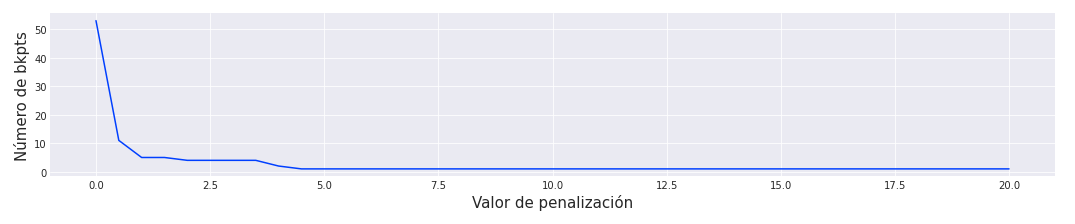
\includegraphics[width=.85\textwidth]{images/5.png}
          \caption{Gráfico de valor de penalización vs número de puntos de cambio para la alerta en estudio.}
        \end{figure}    
      \end{center}

      \begin{center}
        \begin{figure}[h]
          \centering
          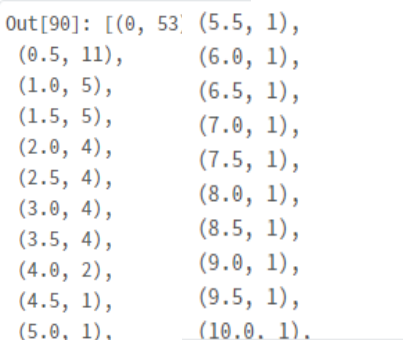
\includegraphics[width=0.3\textwidth]{images/6.png}
          \caption{Tuplas de la forma (\textbf{pen}, \textbf{n\_bkpts}) para la alerta en estudio.}
        \end{figure}    
      \end{center}

    Vemos que el punto de inflexión se da con el valor de penalización 1.0 y tiene asociados 5 puntos de cambio. Con ello, volvemos a correr el modelo ahora con $\text{''pen''}= 1.0$ para visualizar los puntos de cambio:

      \begin{lstlisting}[language=Python]

        # Modelo con el valor de penalizacion escogido

        m_pelt= rpt.Pelt(model="l1").fit(y_mot)
        pen=1.0
        bkpts_pelt = m_pelt.predict(pen=pen)
        
        # Guardamos los puntos de cambio

        breaks = []
        for i in bkpts_pelt:
          breaks.append(df_example_mot["RMS"].index[i-1])
        breaks= pd.to_datetime(breaks)

        print("Los breakpoints son:", breaks)

        # Grafica que muestra los puntos de cambio

        plt.figure(figsize=(12,5.5))
        plt.plot(df_example_mot["fh"], df_example_mot["RMS"])
        plt.title(f'Segmentaciones para pen={pen}')
        print_legend = True
        for i in breaks:
            if print_legend:
                plt.axvline(i, color='red',linestyle='dashed', label='breaks')
                print_legend = False
            else:
                plt.axvline(i, color='red',linestyle='dashed')
        plt.grid()
        plt.legend()
        plt.show()

      \end{lstlisting}

    Luego se tiene la siguiente gráfica con la serie temporal de RMS de la alerta ejemplo y la segmentación generada por sus puntos de cambio:

      \begin{center}
        \begin{figure}[h]
          \centering
          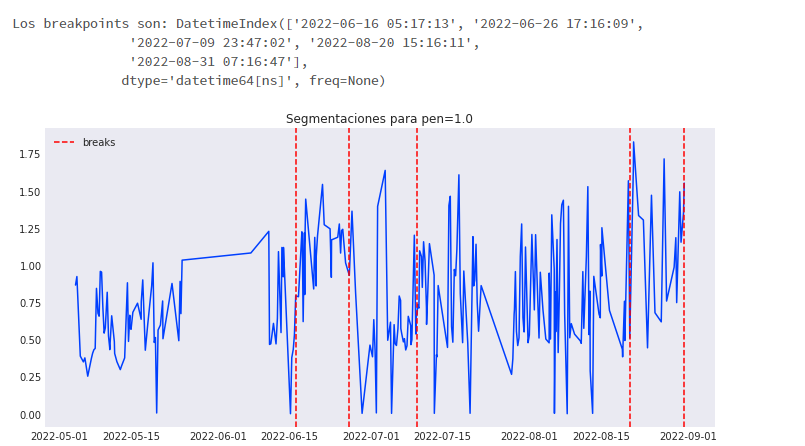
\includegraphics[width=.6\textwidth]{images/8.png}
          \caption{Serie temporal de RMS de la alerta ejemplo segmentada con Pelt}
        \end{figure}    
      \end{center}

    Adicionalmente, se repitió todo el proceso para la serie temporal de RMS diferenciada de la alerta en estudio. Esta transformación permite identificar cambios en la tendencia, eliminar la estacionalidad, estabilizar la varianza y mejorar la estacionariedad de la serie. La transformación se puede realizar rápidamente como sigue: 

      \begin{lstlisting}[language=Python]

        # Creamos la serie diferenciada

        y_mot_diff = np.array(df_example_mot['RMS'])
        y_mot_diff= np.diff(y_mot_diff)
        
      \end{lstlisting}

    En este caso, al realizar el procedimiento para estimar el valor del parámetro de penalización se seleccionó  $\text{''pen''}= 0.5$ y se obtuvieron 4 puntos de cambio.

      \begin{center}
        \begin{figure}[h]
          \centering
          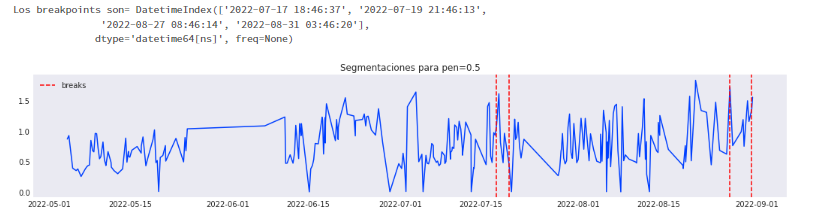
\includegraphics[width=.8\textwidth]{images/22.png}
          \caption{Serie temporal de RMS diferenciada de la alerta ejemplo segmentada con Pelt}
        \end{figure}    
      \end{center}
    
    \subsubsection{Modelos de detección de puntos de cambio con \textit{Opt}}

    Para definir un modelo utilizando el método de búsqueda Opt en Ruptures, debemos considerar una función de costo y el número de puntos de cambio a detectar. La clase \texttt{Dynp} implementa el algoritmo y, al igual que ``Pelt'' posee los argumentos \textbf{model}, \textbf{min\_size} y \textbf{jump}, solo que en este caso se permite utilizar las funciones de costo $L1$, \textit{lineal}, \textit{lineal continua} y \textit{autorregresiva}. Además, \texttt{Dynp} cuenta con el método \textbf{fit(signal)} para ajustar el modelo a la señal en estudio y \textbf{predict(n\_bkps)} para encontrar los puntos de cambio basados en el parámetro del número de cambios a detectar \textbf{n\_bkps}.

    Esta implementación tiene una complejidad computacional del orden $\mathcal{O}(CKn^2)$, donde $K$ es el número de puntos de cambios detectado, $n$ el número de muestras y $C$ la complejidad de llamar a la función de costo considerada en una sub-señal.

    Probaremos modelos con todas las funciones de costo asociadas a los modelos de regresión lineal por partes. En cuanto al número de puntos de cambio a detectar \textbf{n\_bkps}, como no conocemos este valor exacto, seleccionaremos el primer $\text{\textbf{n\_bkps}} \geq 1$ que entregue un segmento final distinto a los anteriormente generados, pues posteriormente se analizarán esos bloques temporales. Tomamos este enfoque dado que un número de puntos de cambio grande puede inducir a segmentaciones pequeñas en las que no se pueda estudiar correctamente el comportamiento de la energía vibratoria de los componentes en estudio. Para ello, se realizó el procedimiento con \textbf{n\_bkps} en un rango de 1 a 10.
    
    El código que genera estos modelos es bastante similar al de Pelt, solo cambiamos la clase Pelt por Dynp y utlizamos el método predict con el argumento \textbf{n\_bkps}. Así, considerando la función de costo $L1$ y la alerta ejemplo vista anteriormente, el modelo se genera de la siguiente manera:

    \begin{lstlisting}[language=Python]

      #Probamos el modelo con distintos valores de numero de puntos de cambio.

      for n_bkps in range(1, 11):
        m_dynp = rpt.Dynp(model="l1").fit(y_mot)
        bkpts_dynp = m_dynp.predict(n_bkps=n_bkps)

        breaks = []
        for i in bkpts_dynp:
            breaks.append(df_example_mot["RMS"].index[i-1])
        breaks = pd.to_datetime(breaks)

        print("Los breakpoints son:", breaks)
        plt.plot(df_example_mot["fh"], df_example_mot["RMS"])
        plt.title(f'Segmentaciones para n_bkps={n_bkps}')
        print_legend = True
        for i in breaks:
            if print_legend:
                plt.axvline(i, color='red', linestyle='dashed', label='breaks')
                print_legend = False
            else:
                plt.axvline(i, color='red', linestyle='dashed')
      plt.grid()
      plt.legend()
      plt.show()

    \end{lstlisting}

    \begin{center}
      \begin{figure}[h]
        \centering
        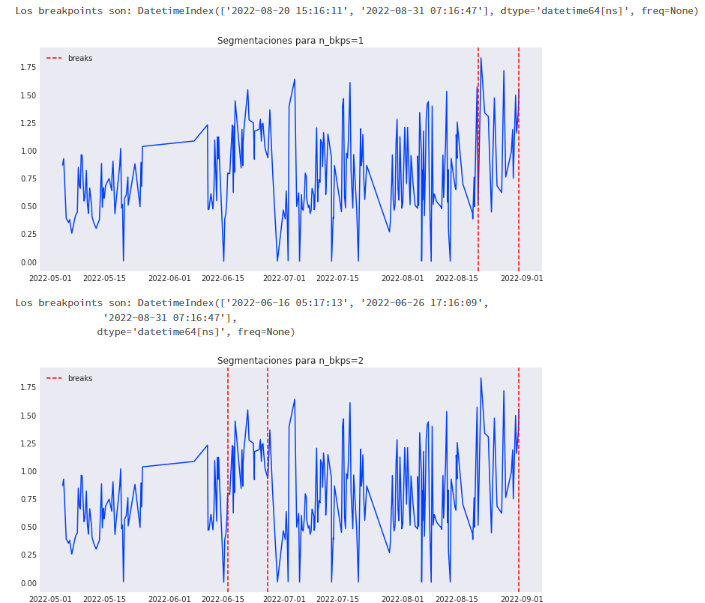
\includegraphics[width=.85\textwidth]{images/25.png}
        \caption{Serie temporal de RMS de la alerta ejemplo segmentada con Opt para $\text{\textbf{n\_bkps}}=1, 2$.}
      \end{figure}    
    \end{center}

    De las gráficas vemos que para $\text{\textbf{n\_bkps}}=1$, el último segmento en la serie temporal coincide con el entregado por el modelo realizado con Pelt y la función de costo $L1$, por lo tanto, en este caso, nos quedaremos con $\text{\textbf{n\_bkps}}=2$. Repetimos este procedimiento con el resto de funciones de costo a probar. Por otro lado, también se realizarán modelos con este método de búsqueda para cada una de esas funciones de costo considerando la serie temporal de RMS diferenciada.

    \subsubsection{Análisis del último bloque temporal y resultados}

    Dado que los modelos estudiados solo encuentran segmentaciones para la serie temporal de RMS de las alertas, no entregan información sobre la validez de estas alarmas de mantenimiento. Es por ello que junto al equipo de Data Science del proyecto establecimos que para cada modelo realizado se analizará el último bloque temporal entregado por la segmentación, buscando comprender qué ocurre justo antes de la generación de la alerta. 

    Este análisis consistirá en ajustar un modelo de regresión lineal y de regresión ponderada para los últimos segmentos temporales. Luego, estudiaremos las pendientes de estos modelos estableciendo que, si la alerta en análisis fue aceptada, la pendiente debería ser significativamente distinta de cero con un nivel de significancia $\alpha= 0, 05$. También evaluaremos el coeficiente de determinación o $R^{2}$, que es una medida que indica la proporción de la variabilidad de la variable dependiente que es explicada por el modelo de regresión. Posteriormente, verificaremos que se cumplan los supuestos principales de los modelos utilizados para ajustar el último bloque temporal.

    A continuación, presentaremos cómo se realizó el análisis del segmento temporal para la alerta ejemplo utilizada anteriormente y considerando el modelo realizado con Pelt, función de costo $L1$ y \textbf{pen}=1.0. Comenzando por el ajuste del modelo de regresión lineal, se usó el siguiente código:

      \begin{lstlisting}[language= Python]

        # Analisis ultimo bloque temporal

        # Obtenemos el segmento para estudiar y lo preparamos 

        ult_bloque= df_example_mot.loc['2022-08-20 15:16:11':'2022-08-31 07:16:47']
        ult_bloque['Time'] = np.arange(len(ult_bloque.index))

        # Creamos el modelo de regresion lineal


        x = ult_bloque.loc[:, ['Time']] 
        y = ult_bloque.loc[:, 'RMS']  
        x = sm.add_constant(x)

        model = sm.OLS(y, x).fit()
        predictions = model.predict(x) 

        print_model = model.summary()
        print(print_model)
        
      \end{lstlisting}

    La regresión ponderada es una técnica que, a diferencia de la regresión lineal, asigna pesos diferentes a los datos según su importancia. Esto ayuda a reducir el impacto de valores atípicos en el ajuste. La implementamos de la siguiente manera:

      \begin{lstlisting}[language= Python]

        # Regresion ponderada

        # Se calculan pesos para una regresion ponderada usando inversos de la 
        # varianza de los residuos.  Luego, se ajusta el modelo de 
        # regresion ponderada con los pesos calculados.

        y_resid = [abs(resid) for resid in model.resid]
        X_resid = sm.add_constant(model.fittedvalues)

        mod_resid = sm.OLS(y_resid, X_resid)
        res_resid = mod_resid.fit()

        mod_fv = res_resid.fittedvalues

        weights = 1 / (mod_fv**2)
        weights

        model_wr = sm.WLS(y, x, weights = weights)
        res_wls = model_wr.fit()

        print(res_wls.summary())
      \end{lstlisting}
    
    La homocedasticidad y la normalidad de los residuos son supuestos fundamentales en un modelo de regresión lineal. La homocedasticidad asegura que la varianza de los errores sea constante, mientras que la normalidad de los residuos indica que estos se distribuyen de manera normal alrededor de cero. Para verificar la homocedasticidad, se utilizó el test de Breusch-Pagan, y para evaluar la normalidad de los residuos, se emplearon los tests de Shapiro-Wilk y Kolmogorov-Smirnov. Los test mencionados son bastante simples de implementar gracias a librerías especializadas:

        \begin{lstlisting}[language= Python]

          # Test de Breusch-Pagan (homocedasticidad)

          name = ["Lagrange multiplier statistic", "p-value", 
                  "f-value", "f p-value"]
          test = sms.het_breuschpagan(model.resid, model.model.exog)
          lzip(name, test)

          # Test de Shapiro-Wilk y Kolmogorov-Smirnov (normalidad)

          print(shapiro(model.resid))
          print(kstest(model.resid, 'norm'))

        \end{lstlisting}

    Notemos que en el caso de la regresión ponderada, dado que permite tener en cuenta la precisión de las observaciones al estimar los coeficientes del modelo, no es necesario estudiar la homocedasticidad y la normalidad de los residuos.

    En resumen, para el ejemplo en estudio se obtuvieron los siguientes resultados:

      \begin{center}
        \begin{figure}[h]
            \centering
            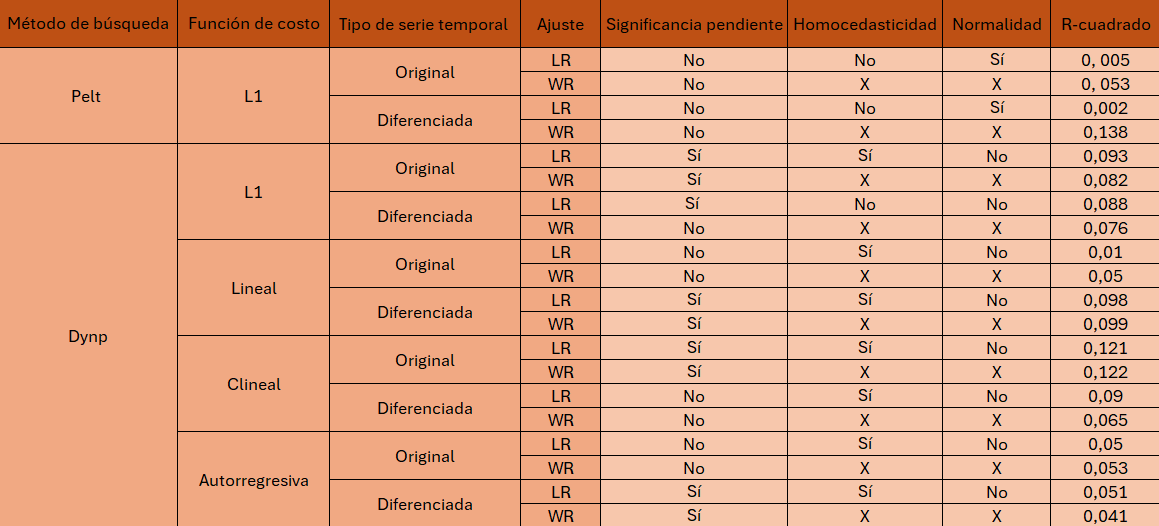
\includegraphics[width=.85\textwidth]{images/results.png}
            \caption{Tabla resumen análisis último segmento de la alerta en estudio.}
        \end{figure}    
      \end{center}
  
    Recordando que la alerta ejemplo que estamos analizando fue rechazada por el analista, esperábamos ver pendientes no significativas. En este sentido, el método de búsqueda Pelt fue consistente al presentar solamente pendientes no significativas, mientras que Dynp tuvo resultados mixtos. Podemos notar que en los ajustes realizados con regresión lineal ningún caso cumplió con los supuestos de homocedasticidad y normalidad simultáneamente. Por otro lado, en general todos los ajustes tuvieron un $R^{2}$ bajo, siendo $R^{2}= 0.138$ el más alto.

    Si bien en un principio la idea era estudiar todas las alertas, la metodología de análisis diseñada no permitió realizar esto de manera eficaz. Así, se optó por analizar una alerta aceptada y una rechazada por tipo de componente (motor, reductor y polea). Contrario a lo esperado, los resultados mostraron que no existía una tendencia clara en cuanto al método de búsqueda y función de costo que proporcionaran los mejores resultados, pues todos los ajustes presentaban valores de $R^{2}$ bajos.

  \subsection{Trend Changepoints (librería Prophet)}

    \subsubsection{Sobre la técnica y la librería}

    Prophet es una librería de código abierto desarrollada por Facebook para el análisis y pronóstico de series temporales. Destaca por su facilidad de uso y su capacidad para manejar una variedad de patrones en los datos. Esta biblioteca permite a los usuarios realizar pronósticos precisos y escalables con mínima configuración, lo que la convierte en una herramienta útil para una amplia gama de aplicaciones, incluida la detección de puntos de cambio. 

    Según el artículo publicado por los desarrolladores de Prophet, S. Taylor y B. Letham \cite{taylor2017prophet}, esta librería se basa en un modelo de descomposición de series temporales con tres componentes: tendencia, estacionalidad y días festivos. Supongamos que $y(t)$ es la serie temporal que queremos estudiar con $t$ un índice temporal, luego su descomposición está dada por:
  
     \begin{equation*}
       y(t)= g(t) + s(t) + h(t) + \epsilon_t.
     \end{equation*}

    Aquí $g(t)$ es la tendencia, $s(t)$ es la estacionalidad y $h(t)$ representa los efectos de los días festivos. El término de error $\epsilon_t$ simboliza cualquier variación particular que no sea acomodada por el modelo y asumimos que $\epsilon_t$ está distribuido normalmente. 

    En Prophet existe una herramienta de detección de puntos de cambio en la tendencia, conocida como Trend Changepoints. Esta herramienta consiste en un algoritmo que busca segmentar la serie temporal en intervalos donde la tendencia es relativamente constante. Para lograrlo, utiliza una función de costo que tiene la siguiente forma:
     \begin{equation*}
       \text{Costo total} = \text{Costo de Ajuste} + \text{Penalización},
     \end{equation*}

    donde $\text{Costo de Ajuste}$ mide la discrepancia entre los datos observados y el modelo ajustado en cada intervalo y $\text{Penalización}$ es una componente que penaliza la cantidad y magnitud de los cambios en la tendencia entre intervalos consecutivos.

    El objetivo del algoritmo detrás de Trend Changepoints es encontrar la partición de la serie temporal que minimiza el costo total. Esto resulta en una segmentación suave de la tendencia con puntos de cambio significativos. 

    El modelo de tendencia segmentada de Prophet se define de la siguiente manera: 

     \begin{equation*}
       g(t) = (k + a(t) \cdot \delta) \cdot t + (m + a(t)\cdot \delta),
     \end{equation*}

    donde $k$ es la tasa de crecimiento base, $a(t)$ es la función indicadora de cambio, $\delta$ es un vector de ajustes de cambio en la tasa de crecimiento, $m$ es el parámetro de desplazamiento y $t$ es el tiempo. 

    La función $a(t)$ se define de la siguiente manera:

     \begin{equation*}
       a(t) = \begin{cases} 
              1 & \text{si } t \geq \text{changepoint} \\
              0 & \text{en otro caso}
              \end{cases}
     \end{equation*}

    La selección automática de los puntos de cambio se logra utilizando una probabilidad a priori dispersa en los ajustes de los puntos de cambio. Comunmente, se modela la priori dispersa sobre los ajustes $\delta$ con una distribución Laplace $(0, \tau)$ donde $\tau$ controla la flexibilidad del modelo en adaptarse a cambios en la tasa de crecimiento.
  
    \subsubsection{Modelo con Trend Changepoints}

      Para identificar los puntos de cambio en la tendencia, Prophet utiliza un algoritmo basado en PELT (Penalized Early-Late Testing), que busca segmentar la serie temporal en intervalos donde la tendencia es relativamente constante. La clase \texttt{TrendChangepoints} de Prophet implementa este algoritmo y tiene los siguientes argumentos asociados:

      \begin{itemize}

        \item \textbf{changepoints (array-like, opcional):} Una lista de fechas en las que se sospecha que hay cambios en la tendencia.
        \item \textbf{changepoint\_range (float, opcional):} Proporción del historial que se utilizará para encontrar los puntos de cambio. Valor por defecto: 0.8.
        \item \textbf{changepoint\_prior\_scale (float, opcional):} Escala de prioridad para el modelo de puntos de cambio. Valor por defecto: 0.05.
        \item \textbf{n\_changepoints (int, opcional):} Número de puntos de cambio que se deben seleccionar. Si no se especifica, se usará el valor predeterminado de Prophet para el número de puntos de cambio.
        \item \textbf{holidays (DataFrame, opcional):} Un DataFrame con las fechas de las vacaciones que se deben considerar en el modelo. El DataFrame debe tener una columna 'holiday' con el nombre de la vacación y una columna 'ds' con la fecha.
        \item \textbf{seasonality\_prior\_scale (float, opcional):} Escala de prioridad para la estacionalidad. Un valor más alto da más peso a la estacionalidad en el modelo. Valor por defecto: 10.
        \item \textbf{holidays\_prior\_scale (float, opcional):} Escala de prioridad para las vacaciones. Un valor más alto da más peso a las vacaciones en el modelo. Valor por defecto: 10.
      \end{itemize}

      Para ajustar el modelo y obtener las predicciones, la clase \texttt{TrendChangepoints} cuenta con los siguientes métodos:

      \begin{itemize}
        \item \textbf{fit(signal):} Ajusta el modelo a la serie temporal de entrada.
        
        \item \textbf{predict(signal):} Devuelve los puntos de cambio óptimos en la tendencia identificados por el algoritmo.
      \end{itemize}

    Ya que este modelo es relativamente sencillo de utilizar, se optó por probarlo con las alertas separadas según su estado. Ejemplificaremos lo realizado para las alertas rechazadas y aceptadas en motores. Se desarrolló un código que las selecciona y obtiene los indicadores asociados a ellas, creando un identificador único para cada alerta rechazada. Se optó por utilizar dos enfoques diferentes para analizar las alertas rechazadas: uno basado en la evolución temporal del RMS normalizado y otro basado en la mediana de las mediciones de RMS normalizadas. La razón detrás de esto es que la mediana es una medida robusta que puede ser menos sensible a valores extremos o fluctuaciones aleatorias en los datos. Al utilizar la mediana en lugar de la evolución temporal, se busca reducir el impacto de posibles ruidos o variabilidades en los datos, permitiendo una mejor detección de patrones o tendencias subyacentes en las alertas rechazadas.

    \begin{lstlisting}[language=Python]

      # Alertas Rechazadas
      len(df_alerts_mot.loc[df_alerts_mot['status']=='Declined'])

      # Como vemos, existen 17 alertas rechazadas.

      # Filtramos para obtener los i_indicadores asociados a alertas rechazadas.
      # Luego se crea un id para cada una de estas alertas (esto debido a que 
      # un i_indicador puede estar relacionado a mas de una alerta)

      tempdf= df_alerts_mot.loc[df_alerts_mot['status']=='Declined']
      tempdf['tempid'] = range(1, len(tempdf) + 1)
      new_temp = tempdf.loc[:, ['i_indicador', 'tempid']]

      # Guardamos en una lista los i_indicadores que se relacionan con alertas 
      # rechazadas, luego obtenemos las mediciones de los sensores con sus fechas. 

      i_indicador_r= new_temp['i_indicador'].tolist()
      declined= df_features_mot[df_features_mot['i_indicador'].isin(i_indicador_r)]

      # Agregamos a las mediciones de RMS, fecha, i_indicador, id_alerta la columna 
      # tempid, que contiene un id para cada alerta rechazada.

      rechazadas = pd.merge(declined, new_temp, on='i_indicador')
      rechazadas['RMS_normalized'] = pp.minmax_scale(rechazadas.loc[ : , 'RMS'], 
      feature_range = (0, 10), axis = 0, copy = True)

      # Crear columna con la fecha

      rechazadas['date'] = rechazadas['fh'].dt.date

      # Columna con la mediana de los RMS normalizados por dia 
      
      rechazadas['mediana']= rechazadas.groupby('date')['RMS_normalized']

      # Ajustamos los nombres de las columnas para el modelo.

      # Para el primer modelo, preparamos las entradas de la fecha y 
      # RMS normalizado.

      rechazadas.rename(columns={'date':'ds', ''RMS_normalized'':'y'}, inplace=True)
      
      # Para el segundo, utilizaremos la mediana del RMS normalizado calculada diariamente.

      # rechazadas.rename(columns={'date':'ds', 'mediana':'y'}, inplace=True)

      # Agrupamos el df anterior segun el id de cada alerta rechazada, luego  
      # creamos una lista de df que contendra las fechas, RMS, i_indicador,  
      # id_alert asociado a cada id de alerta rechazada.

      grupo=rechazadas.groupby(['tempid'])

      ts_r= []

      for name, group in grupo:
            ts_r.append(group)
    \end{lstlisting}

  Del código anteriormente presentado, obtuvimos el siguiente DataFrame resultante para las alertas rechazadas:
    \begin{center}
      \begin{figure}[h]
        \centering
        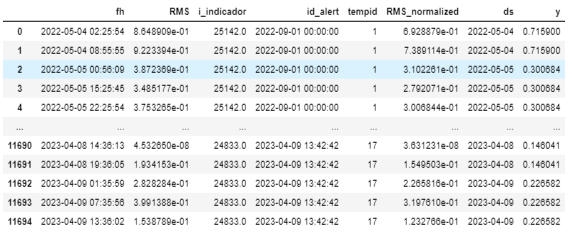
\includegraphics[width=.85\textwidth]{images/94.png}
        \caption{Dataframe consolidado alertas rechazadas en motores.}
      \end{figure}    
    \end{center}
  

  Para aplicar el modelo de Trend Changepoints, se utilizaron los parámetros \textbf{changepoint\_range=1} (pues deseábamos que se analice la serie completa) y \textbf{changepoint\_prior\_scale=0.8}. Este último fue seleccionado utilizando la herramienta de Hyperparameter tuning de Prophet, que evaluó diferentes valores de este hiperparámetro para encontrar aquellos que proporcionaban el mejor rendimiento en términos de métricas como el RMSE. El resto de los parámetros fueron dejados en default. Para cada alerta dentro de las rechazadas, se ajustará el modelo de Trend Changepoints con los parámetros indicados. Posteriormente, se obtendrán elementos para realizar el análisis del último bloque temporal de cada segmentación resultante. A continuación, se adjunta el código desarrollado para cumplir la tarea:

    \begin{lstlisting}[language=Python]

    for df in ts_r: 
        # Ajustar modelo Prophet a cada serie temporal de alertas rechazadas
        m = Prophet(changepoint_range=1, changepoint_prior_scale=0.8) 
        m.fit(df)

        # Obtener el identificador de la alerta rechazada
        column_value = str(df['tempid'].iloc[0])
        
        # Predecir la serie temporal con el modelo ajustado
        in_sample_forecast = m.predict(df)
        
        # Graficar las segmentaciones y puntos de cambio
        fig = m.plot(in_sample_forecast)
        a = add_changepoints_to_plot(fig.gca(), m, in_sample_forecast)
        plt.title(f'Segmentaciones para alerta_rechazada_id={column_value}')

        # Calcular el ultimo cambio de punto significativo
        final_ds = df['ds'].max()
        if len(signif_bkps(m)) > 0:
            final_bkps = signif_bkps(m).dt.date.max()
        else:
            final_bkps = df['ds'].min()

        # Obtener el ultimo bloque de datos hasta la fecha final
        final_bloque = in_sample_forecast.loc[
                       (in_sample_forecast['ds'].dt.date >= final_bkps) &   
                       (in_sample_forecast['ds'].dt.date <= final_ds)]
        
        # Calcular la pendiente e intercepto de la tendencia en el ultimo bloque
        temp_dates = final_bloque['ds'].apply(lambda x: x.timestamp())
        final_bloque['dt_timestamp'] = temp_dates / 86400
        pend, inte = np.polyfit(
                    final_bloque['dt_timestamp'], final_bloque['trend'], 1)
        df['pendiente'] = pend 
        df['intercepto'] = inte

    # Consolidar los resultados en un DataFrame unico
    alertas_rechazadas = pd.concat(ts_r, axis=0, ignore_index=True)
    alertas_rechazadas = alertas_rechazadas.drop_duplicates(subset=['i_indicador',
                        'pendiente', 'intercepto', 'tempid'])
    alertas_rechazadas.drop(['ds', 'y'], axis=1, inplace=True)
    alertas_rechazadas['pendienteabs'] = np.abs(alertas_rechazadas['pendiente'])

    # Mostrar el DataFrame con los resultados
    display(alertas_rechazadas)

    \end{lstlisting}

  \subsubsection{Análisis del último bloque temporal y resultados}

  Una vez que se aplicó el modelo de Trend Changepoints en cada alerta del grupo de alertas rechazadas y aceptadas, se ajustó un modelo de regresión lineal para la tendencia del último bloque temporal de cada segmentación generada. Así, el objetivo será analizar 
  

  \subsection{Resultados generales de la tarea}

\section{Conclusiones}

  \subsection{Principales aprendizajes}  
    
  \subsection{Comentarios personales}  

  \subsection{Conclusiones generales}  


\end{document}
